\documentclass{beamer}
\usepackage[utf8]{inputenc}
\usepackage[T1]{fontenc}
\usepackage[english]{babel}
\usepackage{graphicx}
\usepackage{times}
\usepackage{color}
\usepackage{enumerate}
\usepackage{listings}
\lstloadlanguages{C++}

\lstset{language=C++,
basicstyle=\ttfamily\small,
commentstyle=\ttfamily\small,
keywordstyle=\ttfamily\bfseries\small,
stringstyle=\color{red}\ttfamily\small,
commentstyle=\color{grey}\ttfamily\small,
numbers=left,
numberstyle=\color{violet}\ttfamily\scriptsize,
identifierstyle=\color{blue}\ttfamily\small,
showstringspaces=false,
morekeywords={
}}

\definecolor{darkgreen}{rgb}{0.2,0.5,0.05}
\definecolor{grey}{rgb}{0.4,0.4,0.4}

\graphicspath{{./graphics/}}

\usetheme{CambridgeUS}
%\usetheme{Warsaw}

\title[Slajdy w beamerze]{Slajdy w beamerze -- przykłady}

\author[M. Szpyrka.]{Marcin Szpyrka}

\date[2013]{19.02.2013}

\institute[AGH-UST]
{Wydział EAIiIB\\ 
Katedra Informatyki Stosowanej
}

\setbeamertemplate{itemize item}{$\bullet$}

\begin{document}

\begin{frame}
   \titlepage
\end{frame}

%---------------------------------------------------------------------------

\begin{frame}
\frametitle{Plan prezentacji}
\transblindshorizontal

\begin{enumerate}
\item Wprowadzenie
\item Sieci Petriego niskiego poziomu
\item Kolorowane sieci Petriego
\item RTCP-sieci -- motywacje 
\item Charakterystyka RTCP-sieci
\item Nowy model czasu
\item Dynamika RTCP-sieci
\item Analiza RTCP-sieci
\end{enumerate}
\end{frame}

%---------------------------------------------------------------------------

\begin{frame}
\frametitle{Sieci miejsc i przejść}

\centerline{
\only<1>{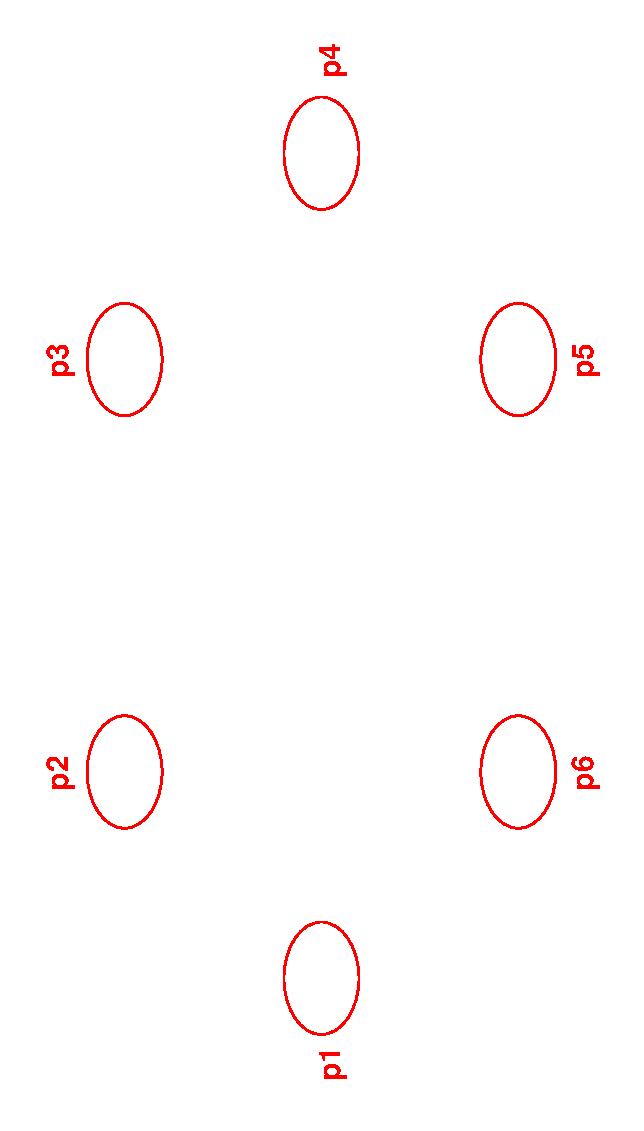
\includegraphics[width=5.3cm,angle=270]{pt-4}}%
\only<2>{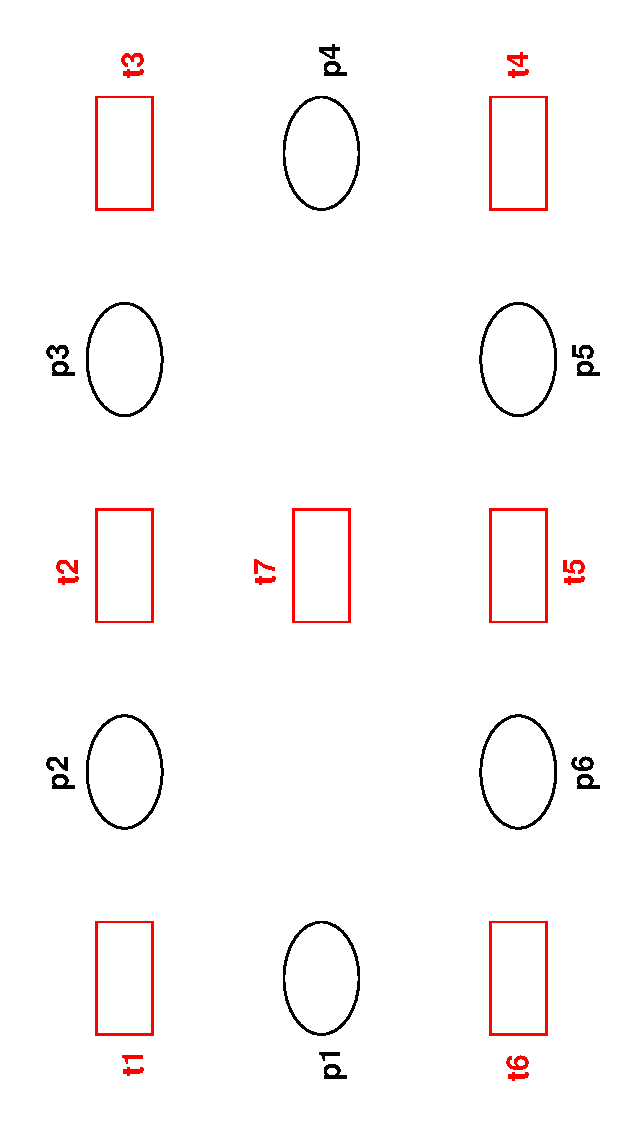
\includegraphics[width=5.3cm,angle=270]{pt-3}}%
\only<3>{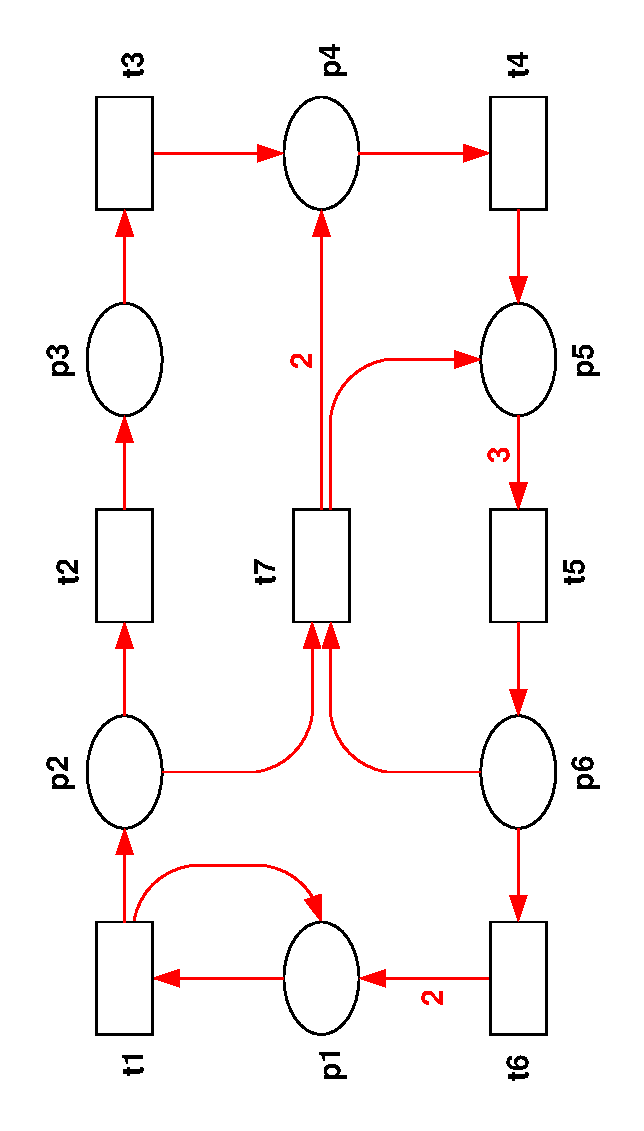
\includegraphics[width=5.3cm,angle=270]{pt-2}}%
\only<4>{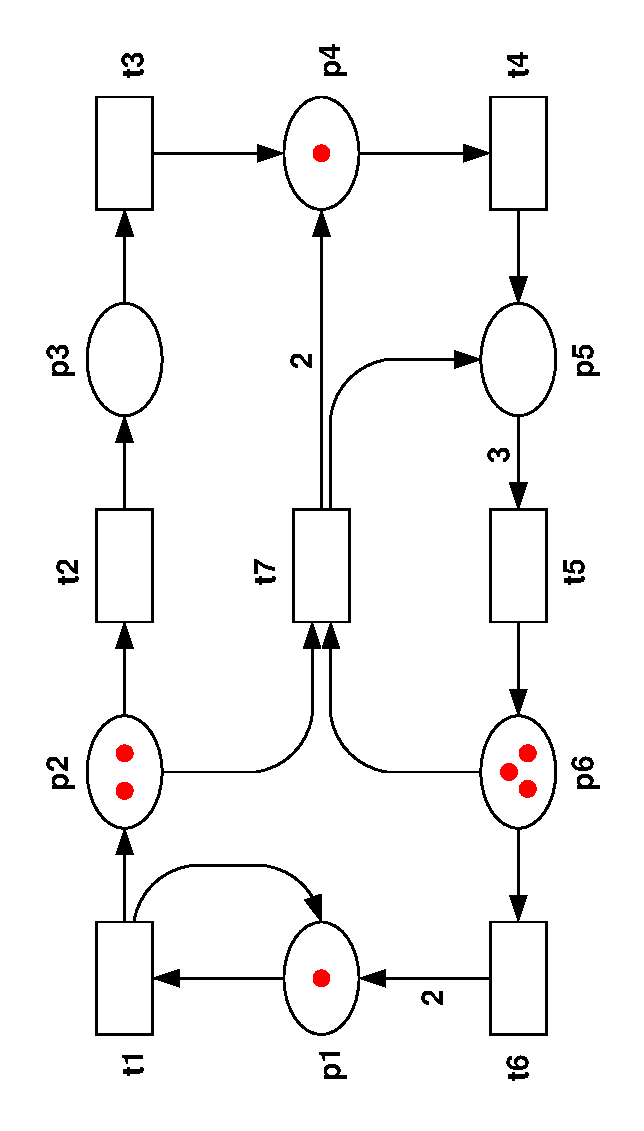
\includegraphics[width=5.3cm,angle=270]{pt-1}}%
\only<5>{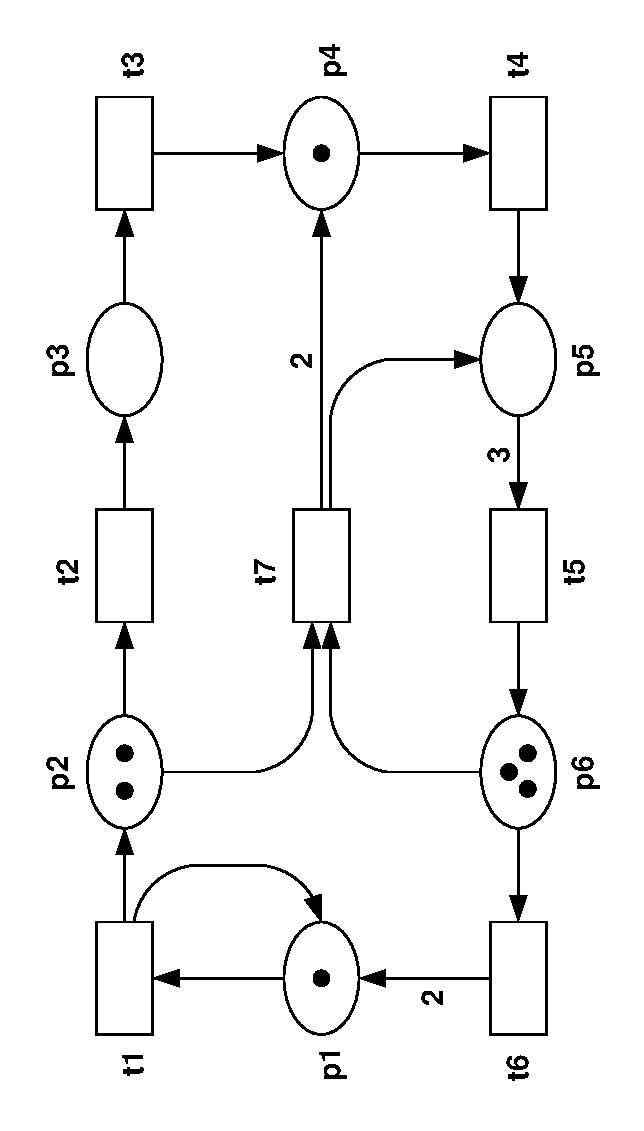
\includegraphics[width=5.3cm,angle=270]{pt1}}%
\only<6>{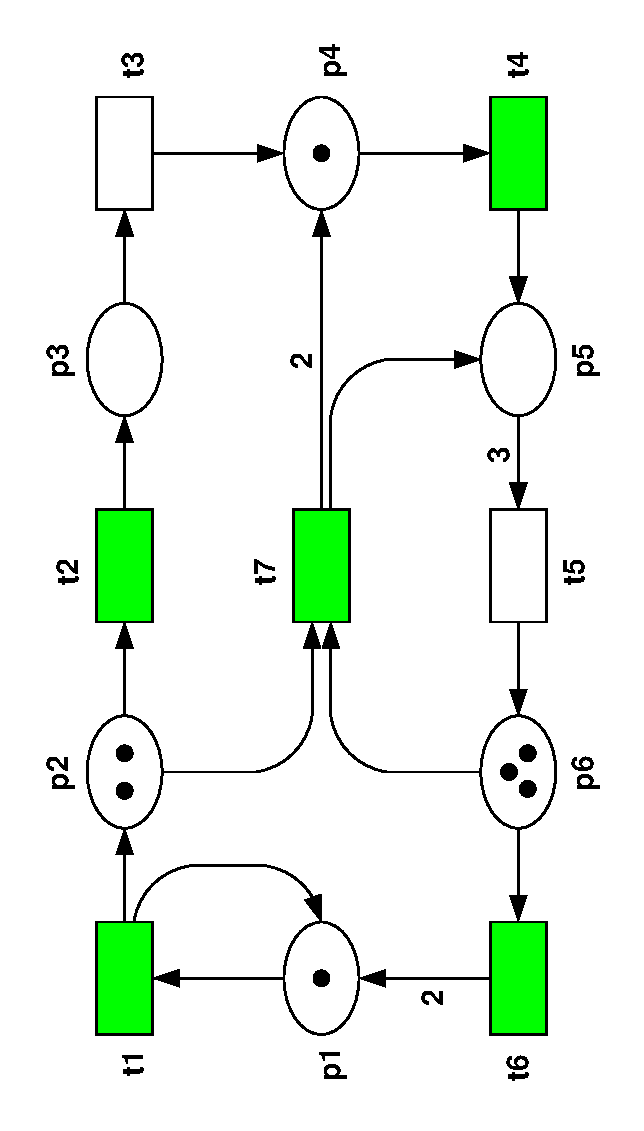
\includegraphics[width=5.3cm,angle=270]{pt2}}%
\only<7>{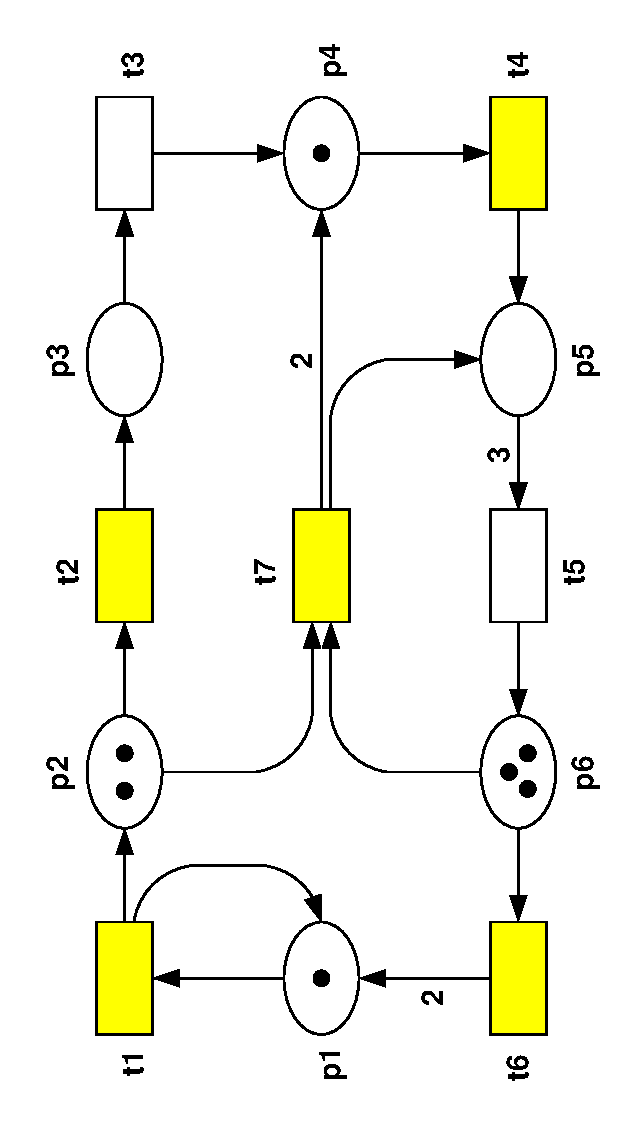
\includegraphics[width=5.3cm,angle=270]{pt3}}%
\only<8>{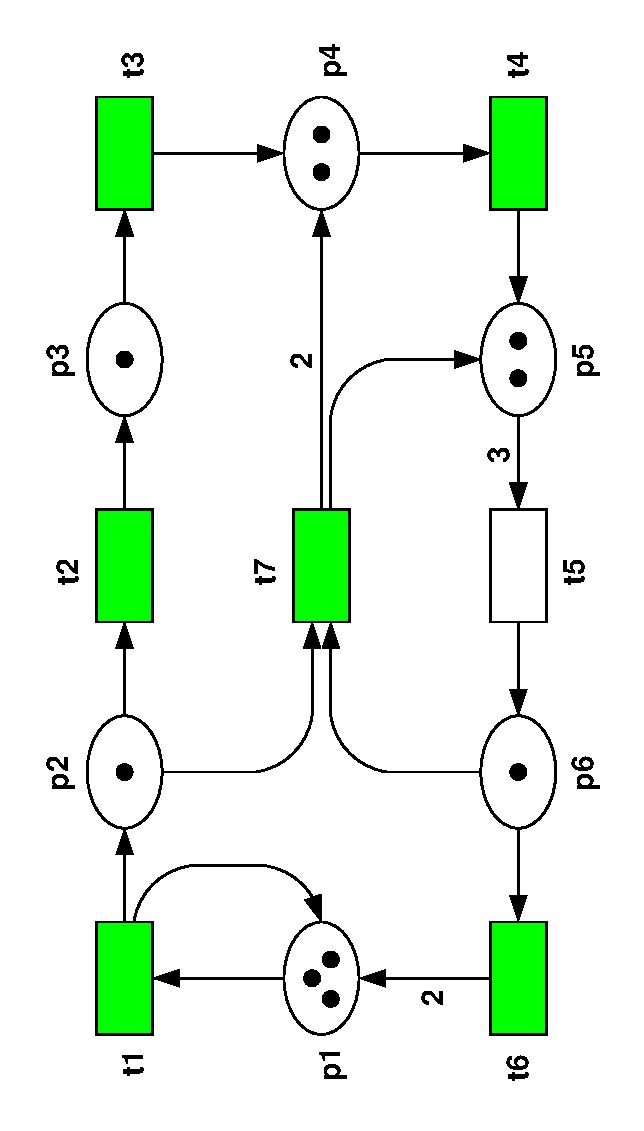
\includegraphics[width=5.3cm,angle=270]{pt4}}%
\only<9>{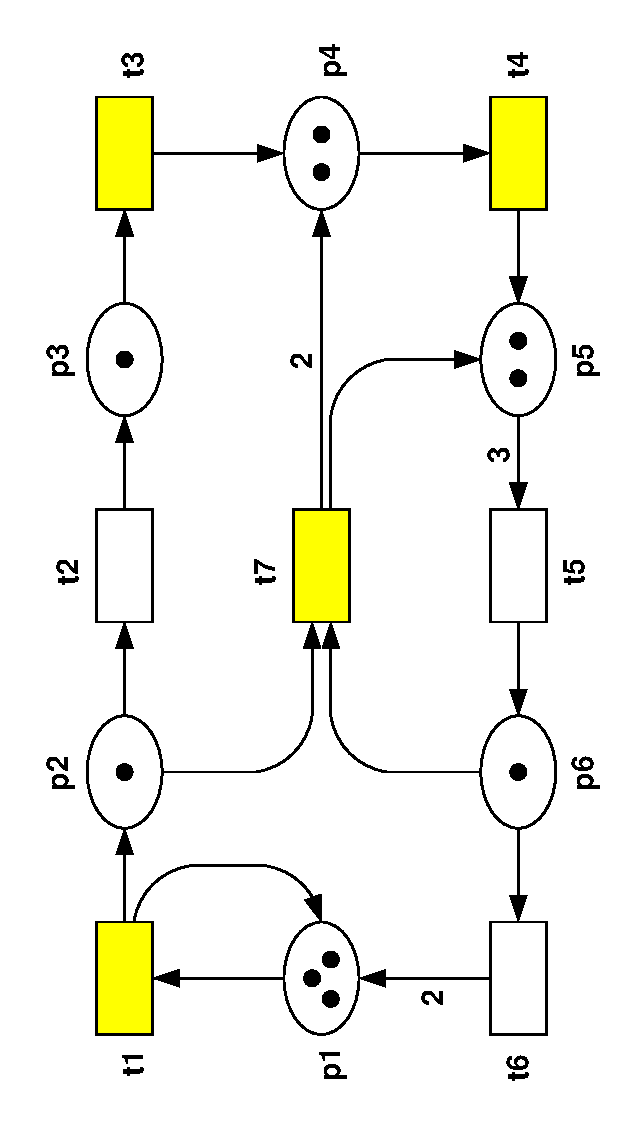
\includegraphics[width=5.3cm,angle=270]{pt5}}%
\only<10>{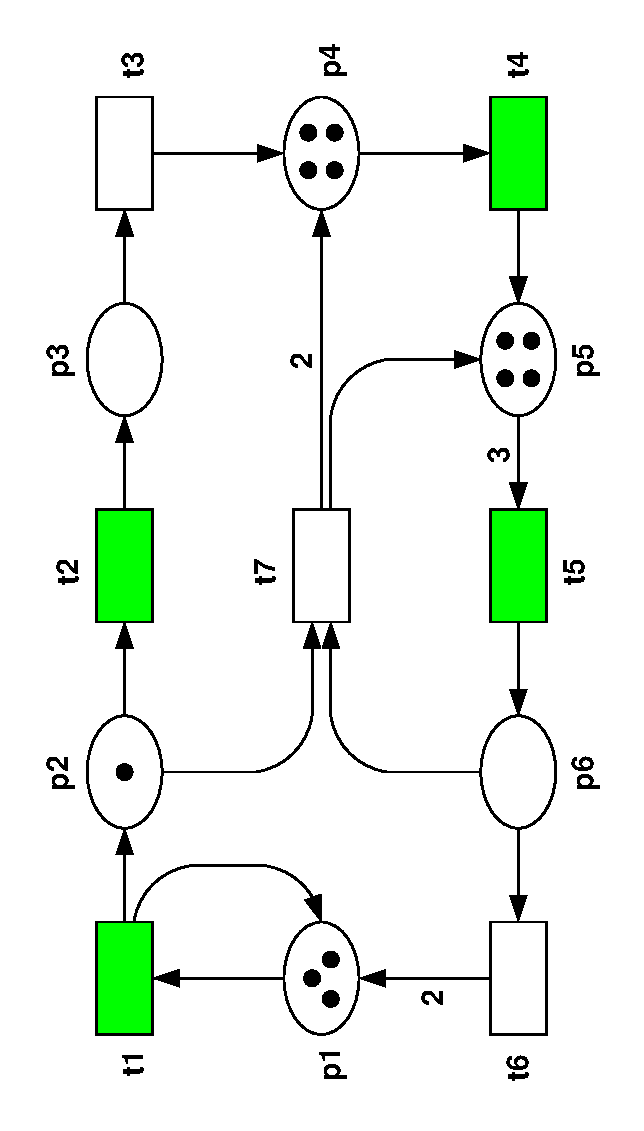
\includegraphics[width=5.3cm,angle=270]{pt6}}%
\only<11>{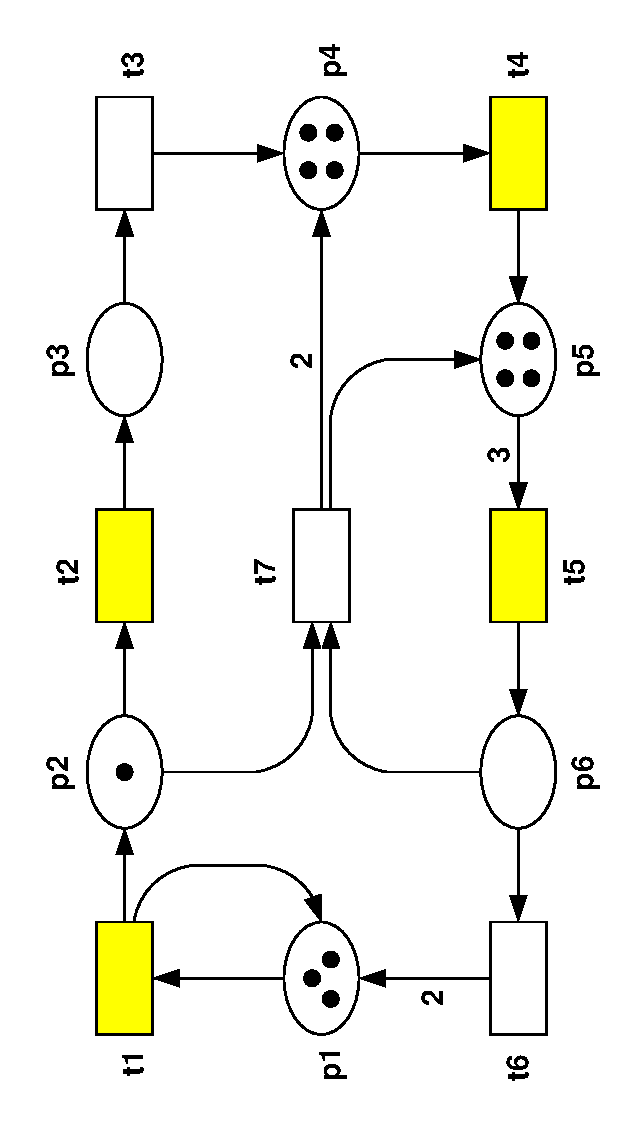
\includegraphics[width=5.3cm,angle=270]{pt7}}%
\only<12>{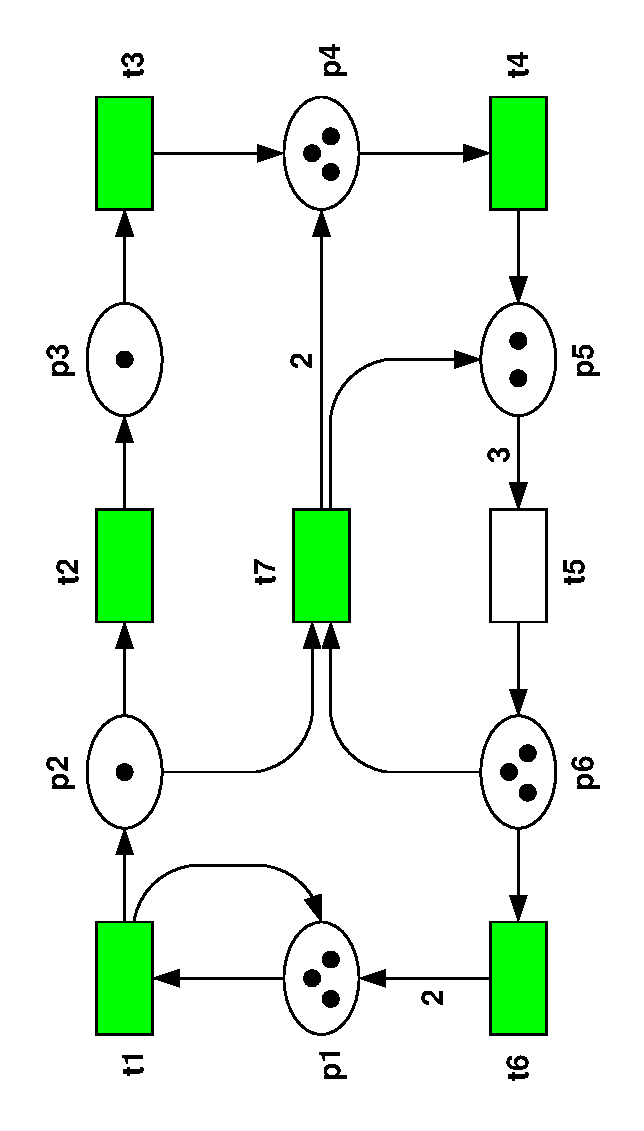
\includegraphics[width=5.3cm,angle=270]{pt8}}%
}

\end{frame}

%---------------------------------------------------------------------------

\begin{frame}
\frametitle{Kolorowane sieci Petriego}

\centerline{
\only<1>{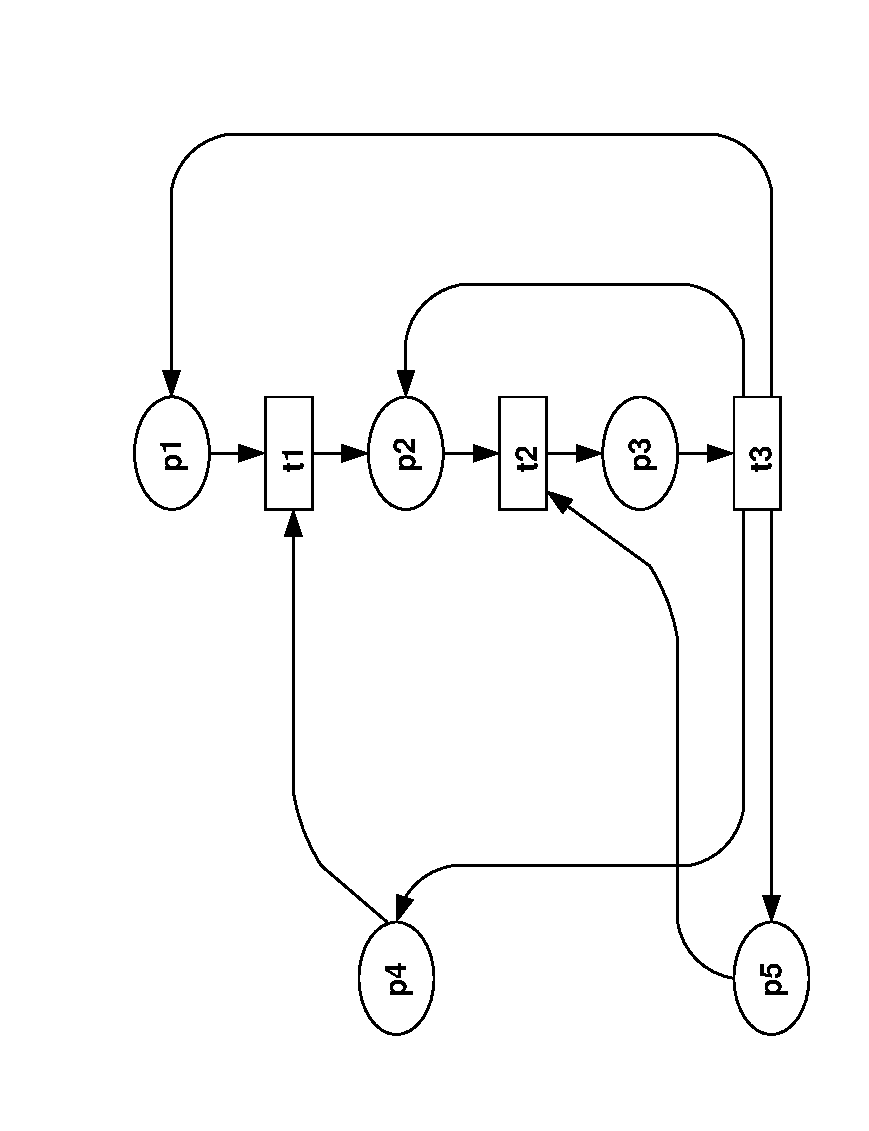
\includegraphics[width=7cm,angle=270]{cp2}}%
\only<2>{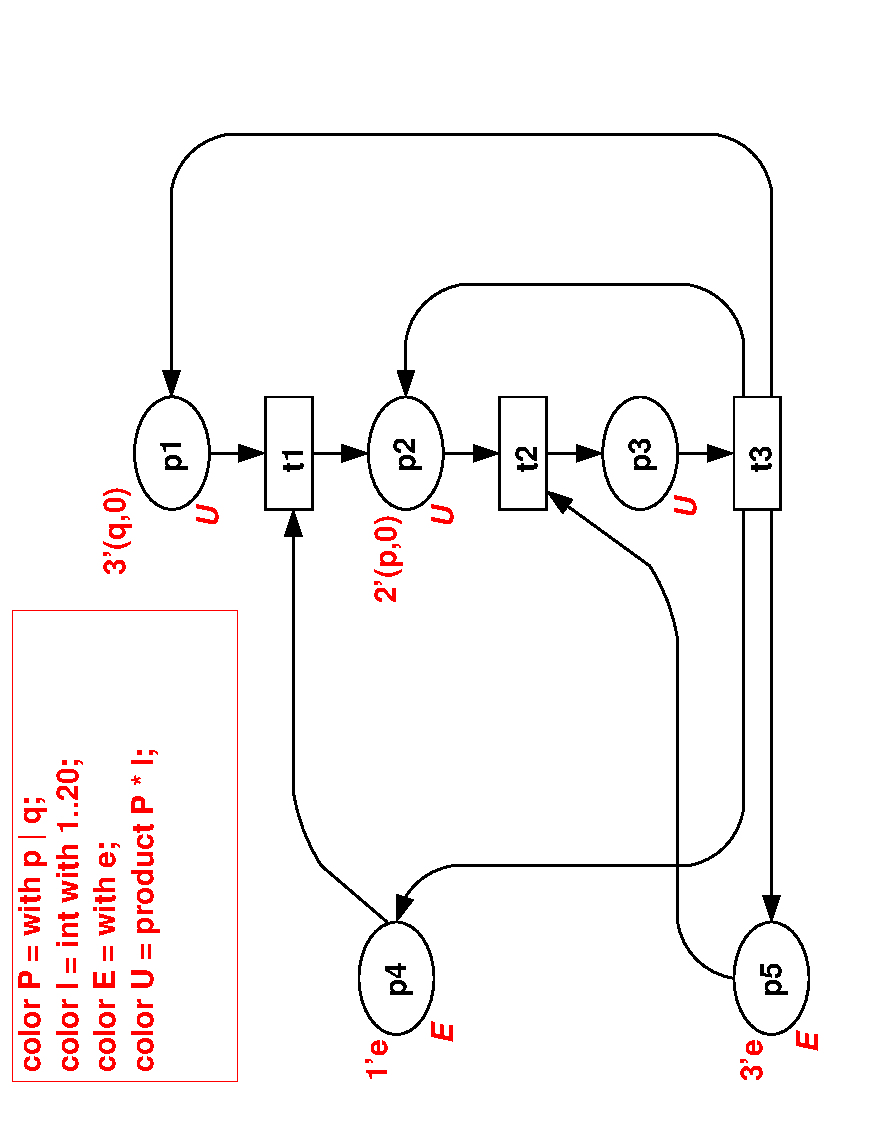
\includegraphics[width=7cm,angle=270]{cp3}}%
\only<3>{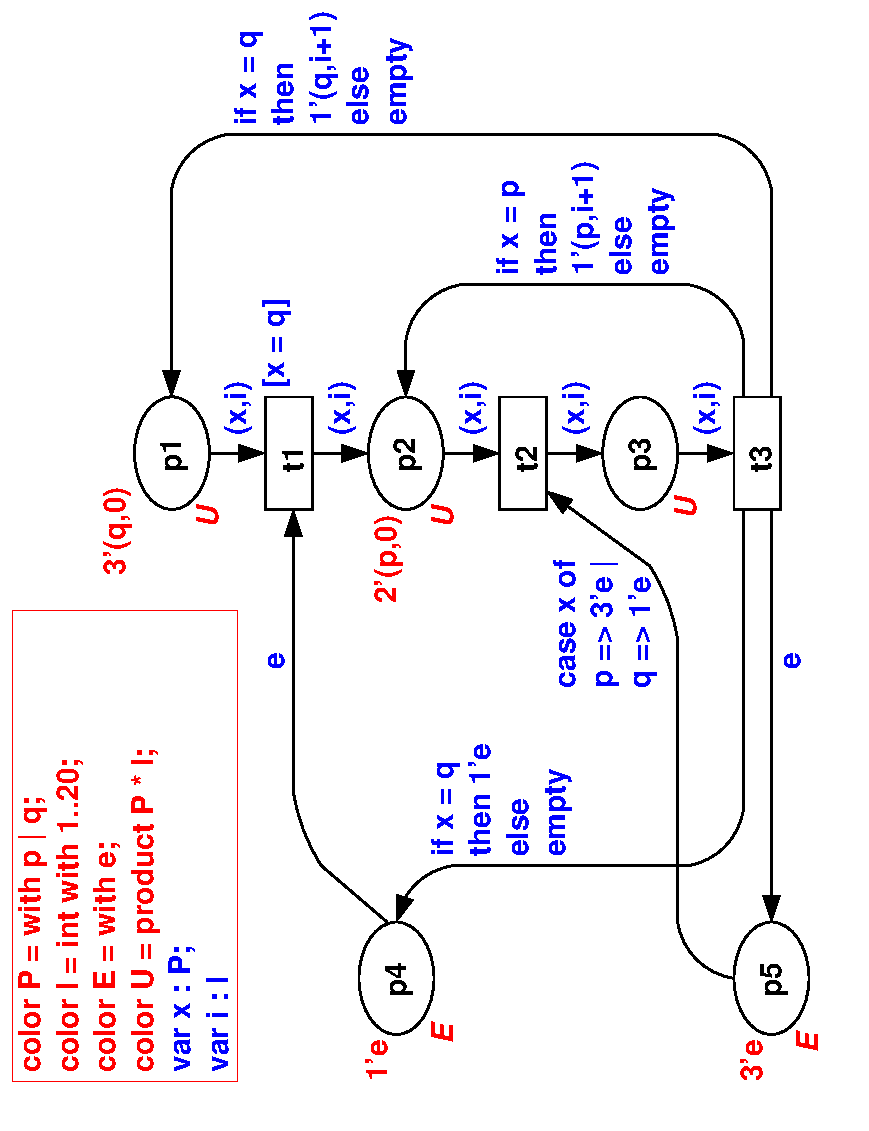
\includegraphics[width=7cm,angle=270]{cp4}}%
\only<4>{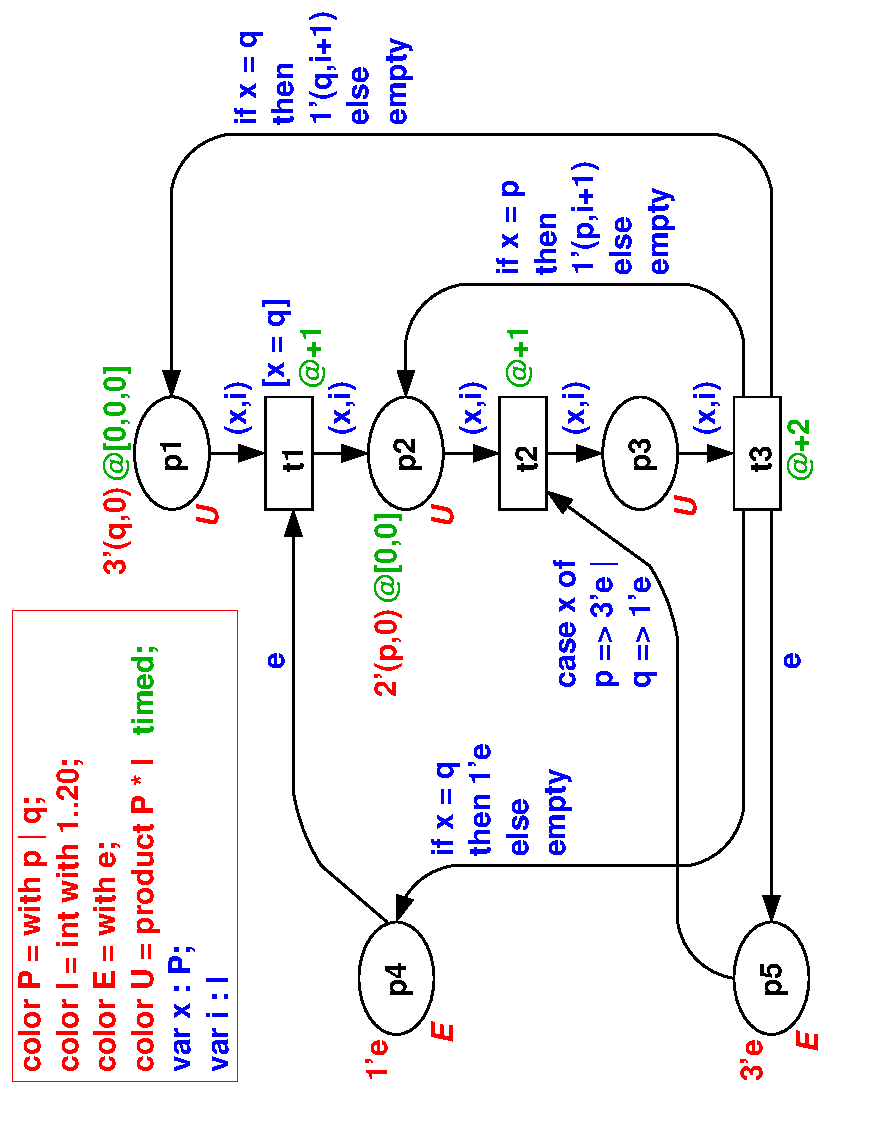
\includegraphics[width=7cm,angle=270]{cp5}}%
}

\end{frame}

%---------------------------------------------------------------------------

\begin{frame}
\frametitle{Zadania}

\centerline{
\only<1>{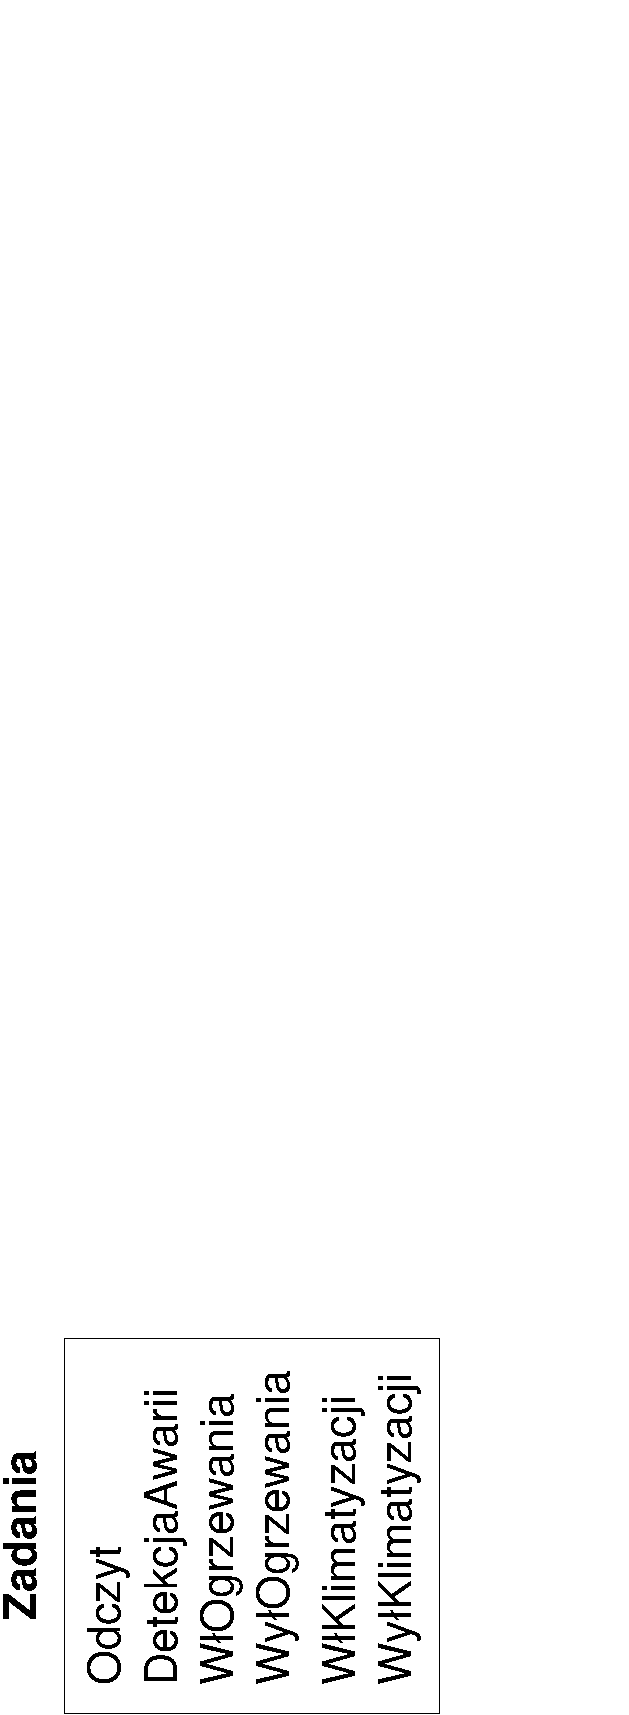
\includegraphics[width=4.2cm,angle=270]{tasksA.pdf}}%
\only<2>{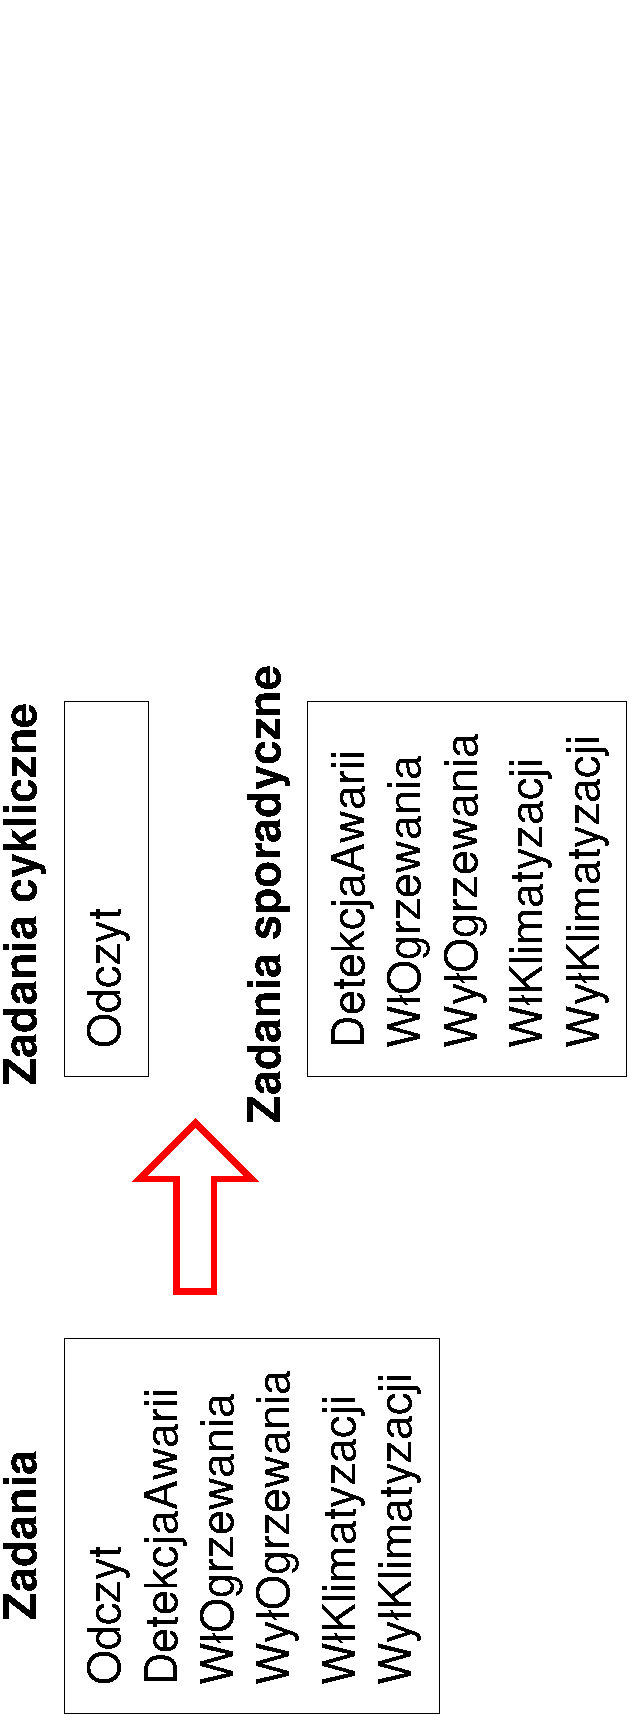
\includegraphics[width=4.2cm,angle=270]{tasksB.pdf}}%
\only<3>{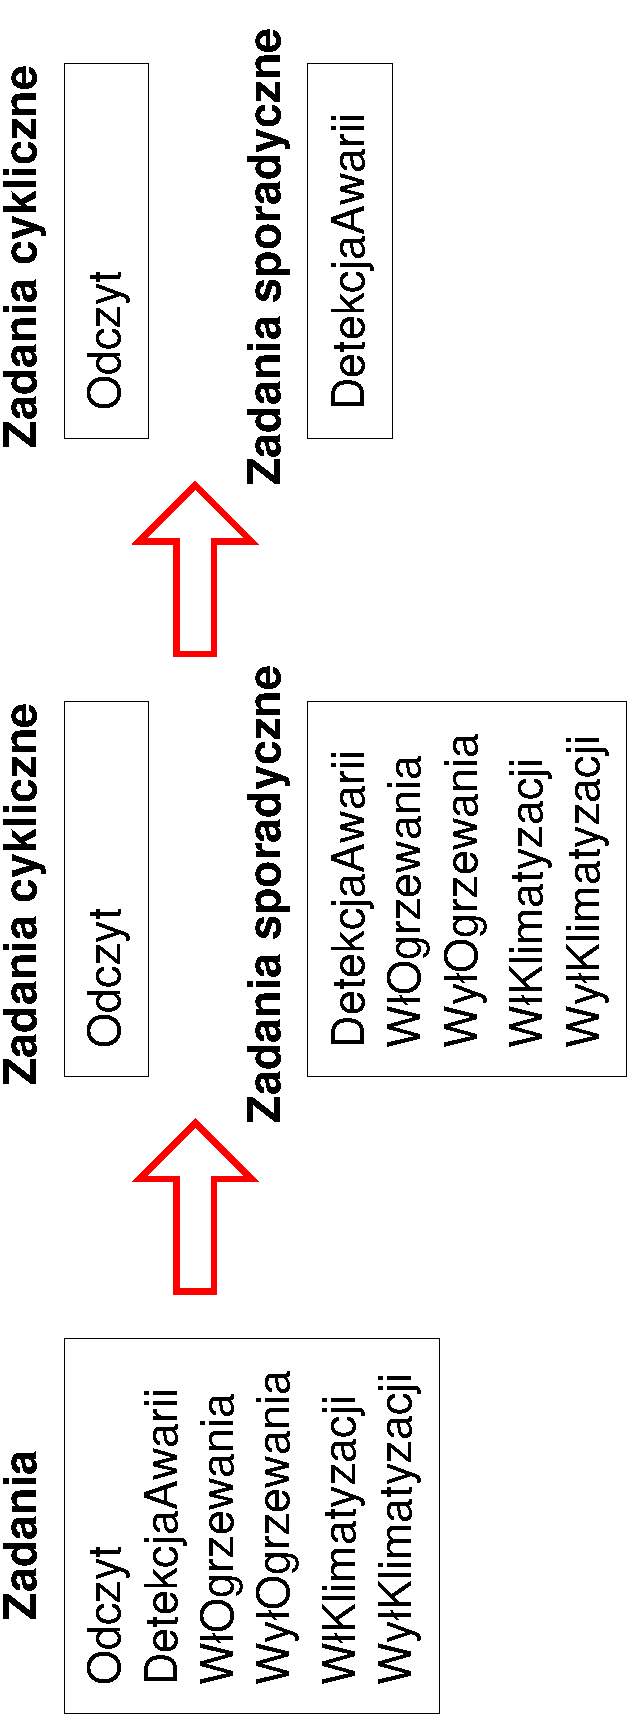
\includegraphics[width=4.2cm,angle=270]{tasksC.pdf}}%
}


\end{frame}

%---------------------------------------------------------------------------

\begin{frame}
\frametitle{CP-sieci vs. RTCP-sieci - podstawowe różnice}

\begin{itemize}
\setlength{\itemsep}{3mm}

\item<1-3>\alert<2>{W~RTCP-sieciach wykorzystywana jest funkcja priorytetów określona na zbiorze przejść sieci.}

\item<2,4>\color<2>{blue}{W~RTCP-sieciach wprowadzono \alert{nowy model czasu}.}

\item<3-> W~RTCP-sieciach niedopuszczalne są łuki wielokrotne, w~przeciwieństwie do CP-sieci, które są multigrafami.

\item<-2> W~RTCP-sieciach, każdy z~łuków ma przypisane dwa wyrażenia: wagę łuku i wyrażenie czasowe. Dowolne wartościowanie wagi łuku musi dawać w~wyniku pojedynczy znacznik odpowiedniego typu, zaś wyrażenia czasowego liczbę rzeczywistą nieujemną. 


\end{itemize}

\only<-2>{\alert{\textbf{RTCP-sieci}}}

\uncover<3->{CP-sieci vs. RTCP-sieci}

\end{frame}

%---------------------------------------------------------------------------


\begin{frame}
\frametitle{CP-sieci vs. RTCP-sieci - podstawowe różnice}

\begin{itemize}[<+->] %[<+-| alert@+>] 
\setlength{\itemsep}{3mm}

\item W~RTCP-sieciach wykorzystywana jest funkcja priorytetów określona na zbiorze przejść sieci.

\item W~RTCP-sieciach wprowadzono nowy model czasu.

\item W~RTCP-sieciach niedopuszczalne są łuki wielokrotne, w~przeciwieństwie do CP-sieci, które są multigrafami.

\item W~RTCP-sieciach, każdy z~łuków ma przypisane dwa wyrażenia: wagę łuku i wyrażenie czasowe. Dowolne wartościowanie wagi łuku musi dawać w~wyniku pojedynczy znacznik odpowiedniego typu, zaś wyrażenia czasowego liczbę rzeczywistą nieujemną. 


\end{itemize}


\end{frame}

%---------------------------------------------------------------------------



\begin{frame}
\frametitle{Stany sieci}

\begin{block}{Znakowanie}
{\em Znakowaniem} sieci $\mathcal{N}$ nazywamy dowolną funkcję $M$ określoną na zbiorze miejsc sieci taką, że:
 \begin{equation} 
\label{eq:znakowanie}
\forall p \in P \colon M(p) \in 2^{C(p)^*}.
\end{equation}
\end{block}

\pause

\begin{block}{Rozkład pieczątek czasowych}
{\em Rozkładem pieczątek czasowych} sieci $\mathcal{N}$ nazywamy dowolną funkcję $S$ określoną na zbiorze miejsc sieci taką, że: 
\begin{equation}
\label{eq:rozkladPieczatek}
\forall p \in P \colon S(p) \in \mathbb{R}.
\end{equation}
\end{block}

\end{frame}

%---------------------------------------------------------------------------



\begin{frame}
\frametitle{Stany sieci}

\begin{columns}
\column{5cm}

\begin{block}{Znakowanie}
{\em Znakowaniem} sieci $\mathcal{N}$ nazywamy dowolną funkcję $M$ określoną na zbiorze miejsc sieci taką, że:
 \begin{equation} 
\label{eq:znakowanie2}
\forall p \in P \colon M(p) \in 2^{C(p)^*}.
\end{equation}
\end{block}

\pause

\column{5cm}
\begin{block}{}
{\em Rozkładem pieczątek czasowych} sieci $\mathcal{N}$ nazywamy dowolną funkcję $S$ określoną na zbiorze miejsc sieci taką, że: 
\begin{equation}
\label{eq:rozkladPieczatek2}
\forall p \in P \colon S(p) \in \mathbb{R}.
\end{equation}
\end{block}
\end{columns}

\end{frame}

%---------------------------------------------------------------------------

\begin{frame}[fragile]
\frametitle{Regulacja dostępu do składowych klasy}

\begin{columns}
\column{0.5\textwidth}
% \begin{block}{}
\begin{lstlisting}
class Point {
private:
  int x;
  int y;
  char name;

public:
  int getX();
  int getY();
  char getName();
  void setX(int i);
  void setY(int i);
  void setName(char c);
  double distance();
};
\end{lstlisting}

% \end{block}

\column{0.35\textwidth}
\begin{figure}[!htb]
\centerline{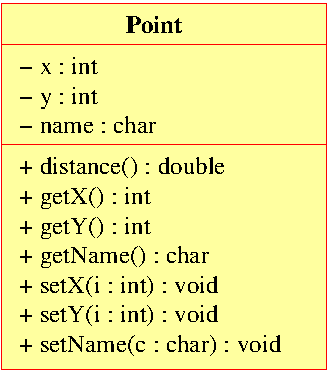
\includegraphics[scale=0.7]{point2}}
\end{figure}
\end{columns}
\end{frame}

%---------------------------------------------------------------------------

\begin{frame}
\frametitle{Alvis}

\begin{columns}
\column{0.1\textwidth}
\column{0.6\textwidth}
\begin{block}{Alvis Language}
\begin{itemize}
  \item Communication Diagrams (AlvisCD)
  \item Alvis Code Language (AlvisCL)
\end{itemize}
\end{block}
\column{0.2\textwidth}
\end{columns}

\vspace{0.6cm}

\begin{columns}
\column{0.2\textwidth}
\column{0.4\textwidth}
\begin{block}{Alvis Toolkit}
\begin{itemize}
  \item Alvis Editor
  \item Alvis Translator
  \item Alvis VM
\end{itemize}
\end{block}
\end{columns}

\end{frame}

%---------------------------------------------------------------------------









\end{document}
%---------------------------------------------------------------------------

